% 저자가 직접 그린 시스템 개요. 슬라이드(images/Frequency_Adapataion.pdf 6쪽)에서
% 벡터로 내보내 잉크 경계로 잘랐다. 그림이 담지 않은 것 -- 두 번째 학습 인코더,
% 헤드 개수, 무엇이 동결인지 -- 는 캡션에 있다.
\begin{figure*}[t]
\centering
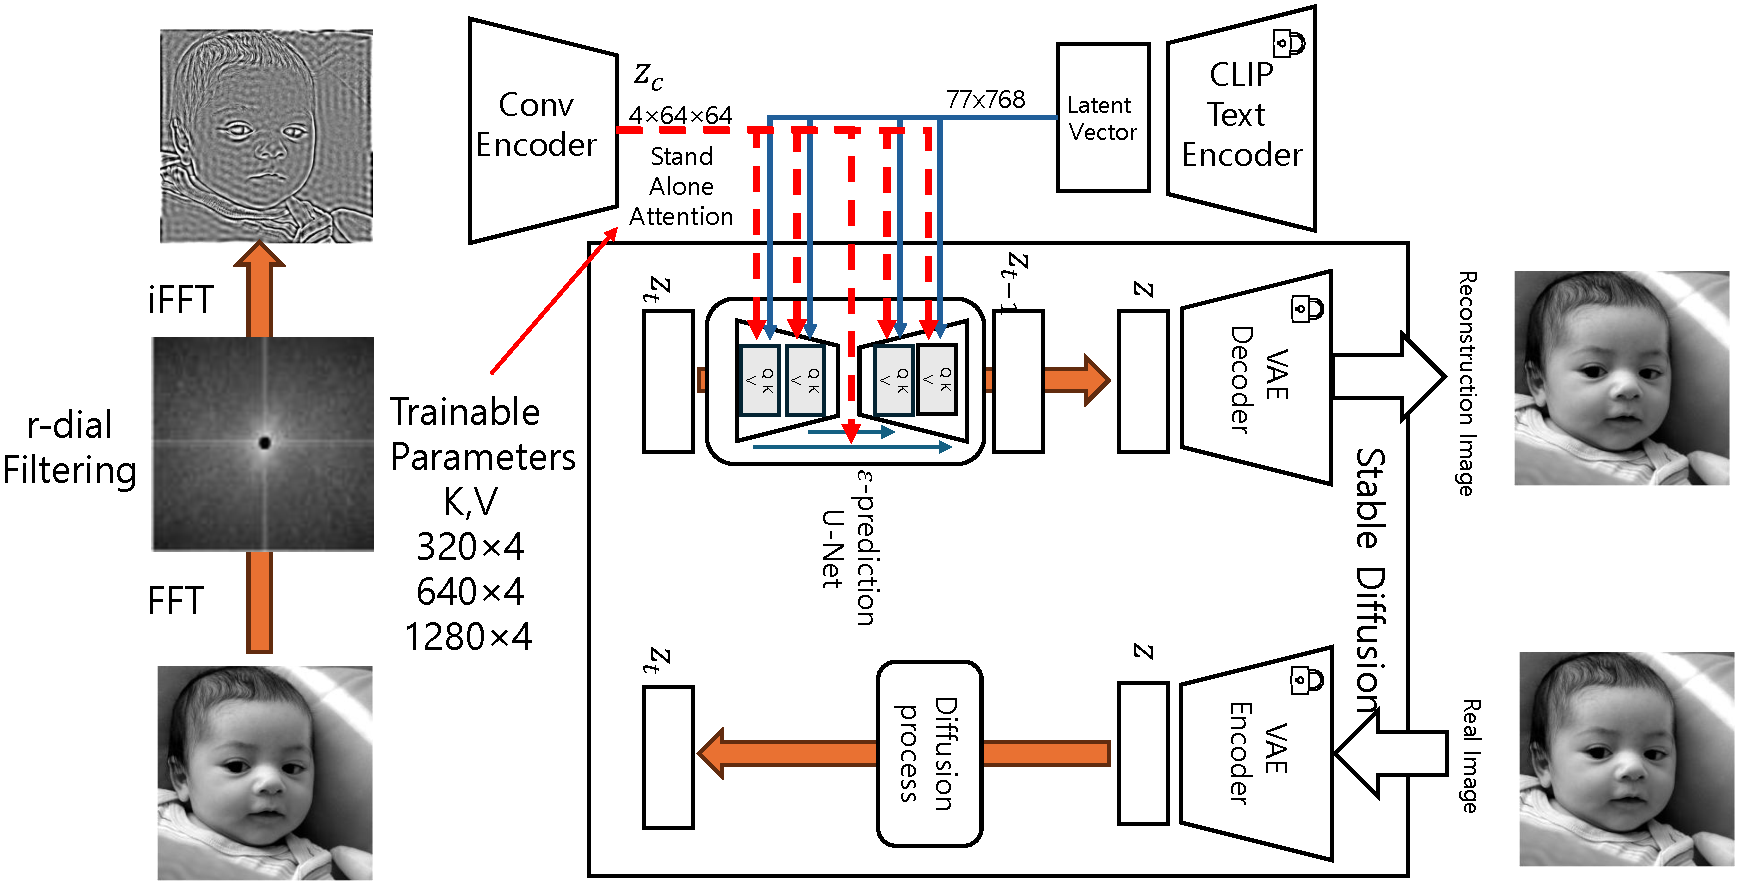
\includegraphics[width=\textwidth]{figures/pipeline}
\caption{반경 $r$의 원판을 스펙트럼에서 제거하고, 학습되는 합성곱 인코더가 그 결과를
전체 해상도로 읽어 VAE를 거치지 않고 4채널 $64{\times}64$의 조건 $z_c$를 만든다. 이는
동결 UNet의 교차 어텐션 16곳으로 들어가며, 그곳에서 학습되는 것은 $W_K$, $W_V$와
0초기화 출력 게이트뿐이고 $W_Q$와 $W_O$는 동결이다(그림~\ref{fig:sa}). 같은 조건 경로의
일부로 그려진 두 번째 학습 stem은 원본 조건을 읽어 디코더 skip 텐서 12곳과 mid block에
0초기화 잔차를 더한다. 구조의 대부분은 그 경로가 나르며, 분배는 측정된 값이다.
$r{=}0$에서 skip 경로만 켜면 SC가 \pathSkipOnlyZero{}, 어텐션만 켜면
\pathAttnOnlyZero{}다(\ref{sec:where}절). 학습은 Min-SNR 가중의 $\epsilon$ 예측이고,
동결 오토인코더를 지나는 루프는 표준 잠재 확산 그대로이며 학습되지 않는다.}
\label{fig:arch}
\end{figure*}
